% !TEX TS-program = xelatex
% !TEX encoding = UTF-8 Unicode

% Lecture Template for ME3001-001-Tristan Hill - Spring 2017 - Fall 2017 - Fall 2020
% Mechanical Engineering Analysis with MATLAB
% Module 3 - Systems of Linear Equations 
% Topic 3 - Existence of Solutions
  

\documentclass[fleqn]{beamer} % for presentation (has nav buttons at bottom)

\usepackage{../analysis_lectures} % sty in the parent directory

\newcommand{\MNUM}{3\hspace{2mm}} % Module number
\newcommand{\TNUM}{3\hspace{2mm}} % Topic number 
\newcommand{\moduletitle}{Systems of Linear Equations} % Titles and Stuff
\newcommand{\topictitle}{Existence of Solutions} 

\newcommand{\sectiontitleI}{Techniques for Solving Linear Systems} % More Titles and Stuff
\newcommand{\sectiontitleII}{Homogeneous and Inhomogeneous Systems}
\newcommand{\sectiontitleIII}{Solution Existence Cases in 2D}
\newcommand{\sectiontitleIV}{Numerical Error and System Condition}


\author{ME3001 - Mechanical Engineering Analysis} 
\title{Lecture Module - \moduletitle}
\date{Mechanical Engineering\vspc Tennessee Technological University}

\begin{document}
	
	\lstset{language=MATLAB,basicstyle=\ttfamily\small,showstringspaces=false}
	
	\frame{\titlepage \center\begin{framed}\Large \textbf{Topic \TNUM - \topictitle}\end{framed} \vspace{5mm}}
	
	% Section 0: Outline
	\frame{
		\large \textbf{Topic \TNUM - \topictitle} \vspace{3mm}\\
		
		\begin{itemize}
			
			\item \sectiontitleI    \vspc % Section I
			\item \sectiontitleII 	\vspc % Section II
			\item \sectiontitleIII 	\vspc %Section III
			\item \sectiontitleIV 	\vspc %Section IV
			
		\end{itemize}
		
	}

\section{\sectiontitleI}

\begin{frame}[label=sectionI] \small 
  \frametitle{\sectiontitleI}
	 \textbf{There are many different techniques for solving linear systems. This is not an exhaustive list.} \\	
	\begin{itemize}
		\item Kramer's Method
		\item Gaussian Elimination 
		\item Gauss-Seidel Method
		\item Jacobi Method
	\end{itemize}
  
\end{frame}

\section{\sectiontitleII}

\begin{frame}[label=sectionII] \small 
  \frametitle{\sectiontitleII}
	 \textbf{ Not all problems can be solved with this type of technique!} \\	
	\begin{itemize}
		\item {\PR non-homogeneous} system is one in which ... \vspace{10mm}\\
		\item most of the time the system will be {\PR non-homogeneous} \vspace{10mm}\\
		\item a {\PR non-homogeneous} system has a {\BL proper solution} if and only if\vspace{2mm}\\
		\[rank(A)=rank([A | b])=n\]
	\end{itemize}
  
\end{frame}

\section{\sectiontitleIII}

\begin{frame}[label=sectionIII] \small 
  \frametitle{\sectiontitleIII}
  {\bf Normal Case - 2 Equations - 2 Unknowns - 1 Solution} \\ \vspace{2mm}
  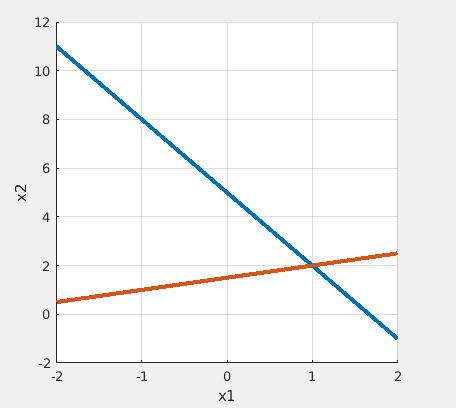
\includegraphics[scale=.3]{lecture5_fig1.png} \\
  \begin{fleqn}
\[3x_1+x_2=5\]
\[x_1-2x_2=-3\]
  \end{fleqn}
\end{frame}
  
\begin{frame}\small  
  \frametitle{\sectiontitleIII}
{\bf Abnormal Case - 2 Equations - 2 Unknowns - $\infty$ Solutions}  \\ \vspace{2mm}
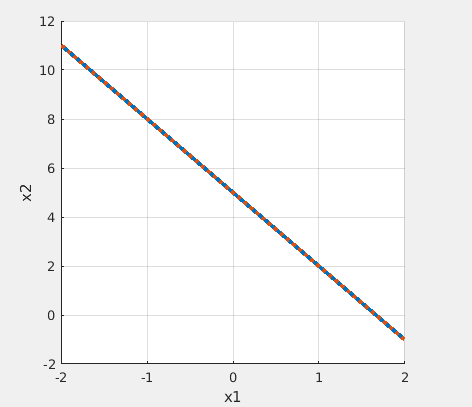
\includegraphics[scale=.3]{lecture5_fig2.png} \\
\begin{fleqn}
\[3x_1+x_2=5\]
\[6x_1+2x_2=10\]
\end{fleqn}
\end{frame}

\begin{frame}\small
  \frametitle{\sectiontitleIII}
{\bf Abnormal Case - 2 Equations - 2 Unknowns - 0 Solutions} \\ \vspace{2mm}
 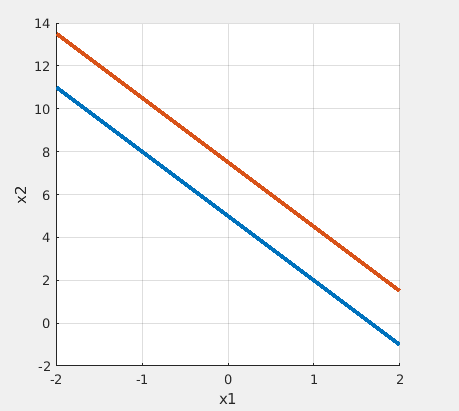
\includegraphics[scale=.3]{lecture5_fig3.png} \\
\begin{fleqn}
\[3x_1+x_2=5\]
\[6x_1+2x_2=15\]
\end{fleqn}
\end{frame}

\begin{frame}\small
\frametitle{\sectiontitleIII}
{\bf Abnormal Case - 3 Equations - 2 Unknowns - 0 Solutions} \\ \vspace{2mm}
 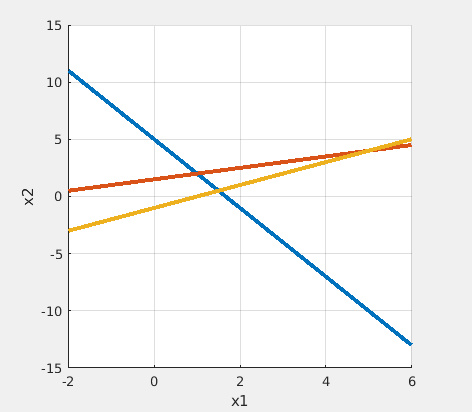
\includegraphics[scale=.3]{lecture5_fig4.png} \\
\begin{fleqn}
\[3x_1+x_2=5\]
\[x_1-2x_2=-3\]
\[x_1-x_2=1\]
\end{fleqn}
\end{frame}

\begin{frame}\small 
\frametitle{\sectiontitleIII}
{\bf Abnormal Case - 3 Equations - 2 Unknowns - 1 Solution} \\ \vspace{2mm}
 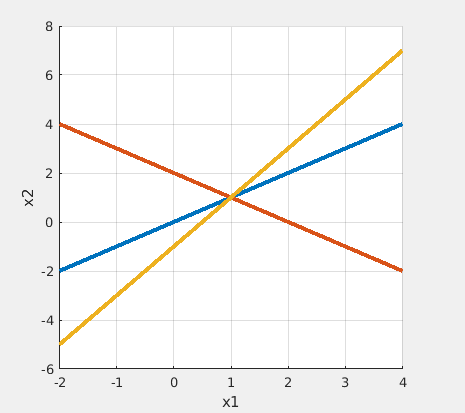
\includegraphics[scale=.3]{lecture5_fig5.png} \\
\begin{fleqn}
\[-x_1+x_2=0\]
\[x_1+x_2=2\]
\[-2x_1+x_2=-1\]
\end{fleqn}
\end{frame}


\section{\sectiontitleIV}

\begin{frame}[label=sectionIV] \small
  \frametitle{\sectiontitleIV}
\textbf{We want our answer to have as little \scalebox{1.5}{error} as possible.} \vspace{3mm}\\

		\textbf{What causes error in the numerical methods?} \\
			``In software engineering and mathematics, numerical error is the combined effect of two kinds of error in a calculation. The first is caused by the finite precision of computations involving floating-point or integer values. The second usually called truncation error is the difference between the exact mathematical solution and the approximate solution obtained when simplifications are made to the mathematical equations to make them more amenable to calculation.''-wikipedia\\
		

\end{frame}

\begin{frame}\small 
  \frametitle{\sectiontitleIV}
	\textbf{Major Causes of Error} \\
		\begin{itemize}
			\item \textbf{floating point computations} \vspace{3mm}\\
			\item \textbf{truncation and solution simplification} \vspace{3mm}\\
			\item \textbf{system condition} \vspace{3mm}\\
		\end{itemize}
		
		 \textbf{ The {\BL System Condition} can cause problems!} \\
\begin{itemize}
	 \item An {\PR ill-conditioned} system can cause error. \\
	
	\item A system is {\PR ill-conditioned} if small changes in the coefficients on the either side of the equation create large variations in the solution.\\
	\end{itemize}
\end{frame}

\begin{frame}\small 
  \frametitle{\sectiontitleIV}
 
\begin{fleqn}
	  
	  Look at this simple 2x2 example. The solution will have huge variations if $ k\approx 1 $. \\
	
		\[x_1 - x_2=5\] 
		\[kx_1 - x_2=4\]
	
	  When $ k = 0.99 $, this gives a solution $(x_1,x_2)=(100, 95)$	
	
		\[x_1 - x_2=5\] 
		\[(0.99)x_1 - x_2=4\]
	
	 When $ k = 1.01 $, this gives a solution $(x_1,x_2)=(-100, 105)$	
	
		\[x_1 - x_2=5\] 
		\[(1.01)x_1 - x_2=4\]
		
\end{fleqn}

\end{frame}

\end{document}

%\begin{document}
%
%\textbf{ \LARGE ME 3001 Lecture - Systems of Linear Equations} \\\\
%\textbf{ \LARGE Solution Existence and Potential Problems } \\
%
%
% \renewcommand\labelitemi{\textbullet}
% \renewcommand\labelitemii{\textendash}
% \renewcommand\labelitemiii{\textasteriskcentered}
% \renewcommand\labelitemiv{\textperiodcentered}
%
%\Large
%\begin{itemize}
%
%\Large
%\item \textbf{ Some problems cannot be solved with this type of technique!} \\	
%\begin{itemize}
%\item {\PR non-homogeneous} system is one in which ... \vspace{10mm}\\
%\item most of the time the system will be {\PR non-homogeneous} \vspace{10mm}\\
%\item a {\PR non-homogeneous} system has a {\B proper solution} if and only if ...\vspace{10mm}\\
%	
%	\scalebox{2}{$rank(A)=rank([A | b])=n\]
%
%\newpage
%\item {\bf Normal Case - 2 Equations - 2 Unknowns - 1 Solution} \\\\ 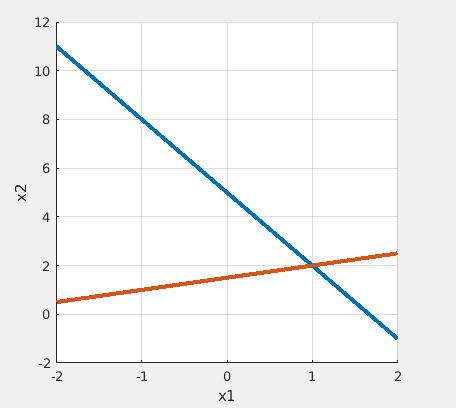
\includegraphics[scale=1]{lecture5_fig1.png} \\\\
%\scalebox{2}{$3x_1+x_2=5\]\\\\
%\scalebox{2}{$x_1-2x_2=-3\]
%
%\newpage
%\item {\bf Abnormal Case - 2 Equations - 2 Unknowns - $\infty$ Solutions} \\\\ 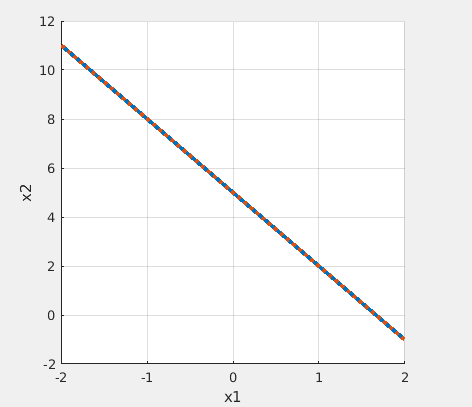
\includegraphics[scale=1]{lecture5_fig2.png} \\\\
%\scalebox{2}{$3x_1+x_2=5\]\\\\
%\scalebox{2}{$6x_1+2x_2=10\]
%
%\newpage
%\item {\bf Abnormal Case - 2 Equations - 2 Unknowns - 0 Solutions} \\\\ 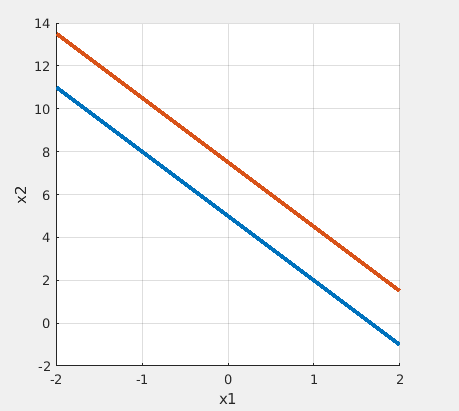
\includegraphics[scale=1]{lecture5_fig3.png} \\\\
%\scalebox{2}{$3x_1+x_2=5\]\\\\
%\scalebox{2}{$6x_1+2x_2=15\]
%
%\newpage
%\item {\bf Abnormal Case - 3 Equations - 2 Unknowns - 0 Solutions} \\\\ 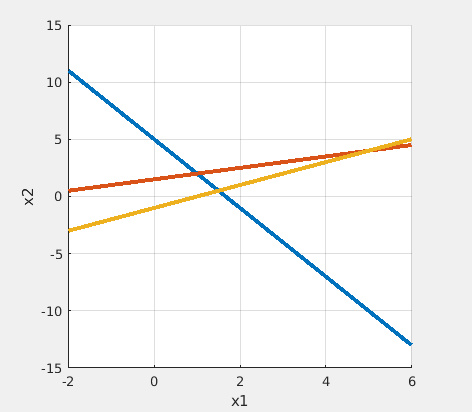
\includegraphics[scale=1]{lecture5_fig4.png} \\\\
%\scalebox{2}{$3x_1+x_2=5\]\\\\
%\scalebox{2}{$x_1-2x_2=-3\]\\\\
%\scalebox{2}{$x_1-x_2=1\]
%
%\newpage
%\item {\bf Abnormal Case - 3 Equations - 2 Unknowns - 1 Solution} \\\\ 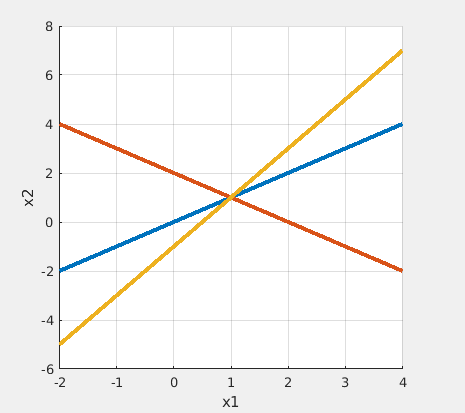
\includegraphics[scale=1]{lecture5_fig5.png} \\\\
%\scalebox{2}{$-x_1+x_2=0\]\\\\
%\scalebox{2}{$x_1+x_2=2\]\\\\
%\scalebox{2}{$-2x_1+x_2=-1\]
%\end{itemize}
%
%\newpage
%\Large
%\item \textbf{ We also want our answer to have as little \scalebox{1.5}{error} as possible.} \\
%	\begin{itemize}
%		\item \textbf{What causes error in the numerical methods?} \\
%			``In software engineering and mathematics, numerical error is the combined effect of two kinds of error in a calculation. The first is caused by the finite precision of computations involving floating-point or integer values. The second usually called truncation error is the difference between the exact mathematical solution and the approximate solution obtained when simplifications are made to the mathematical equations to make them more amenable to calculation.''-wikipedia\\
%		\item \textbf{2 (or 3) Major Causes} \\
%			\begin{itemize}
%				\item \textbf{floating point computations} \vspace{20mm}\\
%				\item \textbf{truncation and solution simplification} \vspace{20mm}\\
%				\item \textbf{system condition} \vspace{20mm}\\
%			\end{itemize}
%	\end{itemize}
%
%\newpage
%\item \textbf{ The {\B System Condition} can cause problems!} \\
%\begin{itemize}
%	\item An {\PR ill-conditioned} system can cause error. \\\\
%	
%	\item A system is {\PR ill-conditioned} if small changes in the coefficients on the either side of the equation create large variations in the solution.\\\\
%
%	\item Let us look at a simple 2x2 example. \\\\
%	
%		\[x_1 - x_2=5\] \\\\
%		\[kx_1 - x_2=4\]\\\\
%	
%	\item The system shown will have huge variations in the solution if \[k\approx 1\]\\\\
%	
%		\[x_1 - x_2=5\] \\\\
%		\[(0.99)x_1 - x_2=4\]\\\\
%	\item When \[k = 0.99\], this gives a solution \[(x_1,x_2)=(100, 95)\]	\\\\
%	
%	\[x_1 - x_2=5\] \\\\
%		\[(1.01)x_1 - x_2=4\]\\\\
%	\item When \[k = 1.01\], this gives a solution \[(x_1,x_2)=(-100, 105)\]	
%
%\end{itemize}
%%\newpage 
%%
%%	 \item \textbf{ \LARGE REMINDER - Homework 3 is posted and is due next Friday !} \\
%% \item \textbf{ \LARGE REMINDER -Exam1 is coming up!} \\
%\end{itemize}
%
%
%	
%
%\end{document}
%
%
%
